% This template found at: https://tex.stackexchange.com/questions/42602/software-requirements-specification-with-latex
% It was a relatively simple template provided by SE user "Yiannis Lazarides"
% whose page is here: https://tex.stackexchange.com/users/963/yiannis-lazarides

%The scrreprt is part of the KOMA-script bundle of packages that does some 
%Fancy-schmancy tweaks to the typography of the resulting document. You know, 
%the kind of stuff that editors and designers love!
\documentclass{scrreprt}

%apparently something is deprecated, but using this package fixes that problem.
\usepackage{scrhack} 

%For code listings
\usepackage{listings}

%I honestly don't know what this is here for. Apparently it addresses some 
%weird edge case having to do with underscores and hyphenation of words. We 
%Could probably do without this package, but perhaps it's required by another 
%package.
\usepackage{underscore}

%How to handle hyperlinks.
\usepackage[bookmarks=true]{hyperref}
\hypersetup{
    bookmarks=true,    % show bookmarks bar?
    pdftitle={Software Requirement Specification},    % title
    pdfauthor={Team Moon Moon},                     % author
    pdfsubject={TeX and LaTeX},                        % subject of the document
    pdfkeywords={TeX, LaTeX, graphics, images}, % list of keywords
    colorlinks=true,       % false: boxed links; true: colored links
    linkcolor=blue,       % color of internal links
    citecolor=black,       % color of links to bibliography
    filecolor=black,        % color of file links
    urlcolor=purple,        % color of external links
    linktoc=all            % all makes whole line a link. "page" -> only page#
}%

%graphics
  \usepackage[pdftex]{graphicx}

%We use these renews so that our enumerations get sublisted with numbers 
%rather than letters.
\renewcommand{\labelenumii}{\theenumii}
\renewcommand{\theenumii}{\theenumi.\arabic{enumii}.}

\def\myversion{0.1.0 }
\title{%
\flushright
\rule{16cm}{5pt}\vskip1cm
\Huge{SOFTWARE REQUIREMENTS\\ SPECIFICATION}\\
\vspace{2cm}
for\\
\vspace{2cm}
Online Postage Ordering System\\
\vspace{2cm}
\LARGE{Release 0.1.0\\}
\vspace{2cm}
\LARGE{Version \myversion approved\\}
\vspace{2cm}
Prepared by Team Moon Moon\\
\vfill
\rule{16cm}{5pt}
}

\date{}

\usepackage{hyperref}
\author{Team Moon Moon}

\begin{document}
\maketitle
\tableofcontents

\chapter*{Revision History}

\begin{enumerate}
\item Team Moon Moon Needs No Revisions.
\item Team Moon Moon Never Makes No Mistakes.
\item Correction. Team Moon Moon ``fails fast.'' Isn't that the new 
buzzword or buzzphrase?
\item The skeleton has been updated to reflect the actual requirements 
provided by Dr. Seaman.
\item It's all really coming together now.
\item Final Revision for Turn-In
\end{enumerate}

\chapter{Introduction}

\section{Purpose}

The purpose of this document is to present a detailed description of the
specifications and the requirements for a postage printing website. It will
explain the purpose and features of the system, the interfaces of the system,
what the system will do, the constraints under which it must operate, and how
the system will react to interactions. This document is intended for both the
stakeholders and the developers of the system.

\section{Project Scope and Product Features}

The objective of this project is to create and implement a website for printing
mailing labels containing USPS postage. The website will be used primarily by
registered users. The website will allow users to: 

\begin{itemize}
\item Create and maintain individual secured accounts
\item Buy/print postage labels
\item List postage purchase history
\item Check account balance
\item Calculate postage rates
\item Track packages
\item Request refunds
\item Check if an address is valid
\end{itemize}

\section{Defintions, Acronyms, and Abbreviations}

At this time, there are no specialized terms in need of definition.

\section{References}

IEEE. IEEE Std 830-1998 IEEE Recommended Practice for Software Requirements
Specifications. IEEE Computer Society, 1998.

\section{Overview}

The second section, the Overall Description, of this document gives an overview
of the products functionality. It describes the informal requirements and is
used to establish a context for the requirements specification in the third
section.

The third section, Requirements Specification, of this document is written
primarily for the developers. It describes details of product functionality. 

\chapter{Overall Description}

This chapter provides an overview of the software product from the perspective 
of the functions that the user is expected to have available to him.

\section{Product Perspective}

The overall idea is that the user may print pre-labelled postage from a
website. The website provides an address verification service, and is licensed
by the relevant governments to sell postage that the relevant governments’
postal services will honor. This makes obtaining and labelling postage much
quicker than by traditional means, wherein one had to drive to the post office
to obtain stamps, and had no way to verify the existence of any particular
address. As well, the user can either add credit to the website or purchase
postage on a one-off basis, and can access a record of all transactions made
with the website.

%\begin{figure}[H]
%\centering
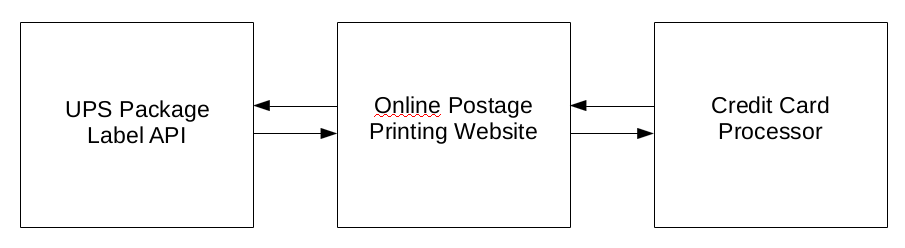
\includegraphics[scale=.4]{2-1-product-perspective.png}
%\label{sec_2_1}
%\end{figure}

\section{Product Functions}

The following subsections detail the various functions that the user of the 
software must be able to utilize.

\subsection{Create An Account}

The Create Account function shall allow a user to create a secure account. The
account will track the user’s full name, mailing address, email address, credit
card information, username and password, and the purchase history for up to two
years.

\subsection{Print Postage}

The Print Postage function shall allow the user to print postage that has been 
purchased, \emph{directly to a printer and NOT to a file.} The postage label 
will be provided upon successfully calling the UPS API, which will return an 
image suitable for printing. 

\subsection{Buy Postage}

The Buy Postage function shall allow the user to purchase postage, using
available credit on their account. Upon a successful print, the user's account 
balance is appropriately debited.

\subsection{List Postage Transactions}

The List Postage Transactions function shall allow the user to view a list of
all of the postage labels that they have printed, including the information
printed on the label, over the past two years.

\subsection{Get Postage Balance}

The Get Postage Balance function shall allow the user to obtain their current
amount in their postage buying account.

\subsection{Calculate Postage}

The Calculate Postage function shall allow the user to enter a name, address,
package type, mail class, and weight. The user shall then be able to see a
calculated postage amount to ship their package.

\subsection{Track/Confirm Package}

The track/confirm package function shall allow users to enter in a tracking
number to see the status of their package. The status of the package will be
received from USPS  and displayed to the user. 

\subsection{Login/Password Reset}

The login function shall allow account members to enter their username and
password.  When verified with the system database, users will be able to access
restricted functions. The login function shall provide users an option to
reset their password. 

\subsection{Refund Request}

The Refund Request function shall allow the user to enter a date and to select
from a list any postage purchase made on that date that they wish to refund as
long as it is not older than ten days old.

\subsection{Validate Address}

The Validate Address function shall allow the user to enter an address to
verify its validity.

\subsection{Logout}

The logout function shall allow the account user to exit out of their account
for security.

\section{User Characteristics}

Users are expected to be Internet literate and be able to navigate in a
website.

\section{Constraints}

While the system does not have any restricting hardware or software
constraints, the system does have some constraints on the user which are
described in the 2.3 User Characteristics part of this document.

\section{Assumptions and Dependencies}

It is assumed that the end user: 

\begin{itemize}
\item Has an Internet connection. 
\item Has a web browser able to display the website.
\item Has a printer.
\end{itemize}

\chapter{Specific Requirements}

\section{External Interface Requirements}

This section details any significant interfaces that the Online 
Postage Printing Website will encounter.

\subsection{System Interfaces}

There are two main system interfaces:

\begin{enumerate}
\item The online credit card processing system. The website will 
access this system via an API to charge cards.
\item The UPS postage label API. The website will make several 
queries to the UPS' APIs in order to calculate shipping cost and 
retrieve labels.
\end{enumerate}

\subsection{User Interfaces}

The system shall provide users access to the USPS postage printing website via
the Internet. There will be two different user interfaces that will accompany
the website: Registered users, and Non-Registered users.

Non-Registered Users: The user will be allowed to register for an account.
The user shall be allowed access only to the follow functions:

\begin{enumerate}
\item Create an Account
\item Track/Confirm Package
\item Validate Address
\end{enumerate}

Registered Users: The user must be logged in at all times. 
The user shall be allowed access to any of the following functions:

\begin{enumerate}
\item Login
\item Print Postage
\item Buy Postage
\item List Postage Transactions
\item Get Postage Balance
\item Refund Request
\item Track/Confirm Package
\item Validate Address
\item Log out
\end{enumerate}

\subsection{Hardware Interfaces}

All hardware shall be required to connect to the internet.

\subsection{Software Interfaces}

There are no special software interface requirements outside of the 
APIs mentioned in the System Interfaces subsection.

\subsection{Communication Interfaces}

There are no special communications interfaces requirements.

\section{Functional Requirements}

The following subsections describe, in detail, the requirements for 
the system in order to provide each function described in section 
2.2.

\subsection{Create an Account}

\begin{enumerate}
\item The user is prompted by the system to provide the following:
\begin{itemize}
\item Full Name
\item Mailing Address
\item Email Address
\item Credit Card Information (Refer to Section 3.4)
\item Unique Username
\item Password
\end{itemize}
\item Once the user has entered the required information, the system verifies
that the required attributes are present, that the email address has a valid
form, that the login name does not exist in the database, and that the password
meets the following criteria:
\begin{itemize}
\item Must be at least 10 characters long
\item Must contain at least one letter
\item Must contain at least one digit
\item Must contain at least on special character (@,\#,\$,\%)
\end{itemize}
\item If the system detects invalid registration information (Required fields
are empty, email address does not have a valid format, the login name is
already in use, or the passwords do not match) then the system shall prompt the
user to reenter the information.  
\begin{itemize}
\item All provided information, entered by the user, should be stored in the
system (Refer to section 3.4).
\end{itemize}
\end{enumerate}

\subsection{Print Postage}

The system shall...

\begin{enumerate}
\item First, ensure
\begin{enumerate}
\item that there is a valid, logged-in user requesting to buy postage.
Otherwise, redirect to the Log In function.
\end{enumerate}
\item Then, provide the user with options of what sort of postage to print 
for. Specifically, provide specific options for class and type, and permit 
the user to enter a number for weight.
\item Then, upon the user selecting a package class, type, and weight, 
request sender and recipient addresses. Proceed to the verify address function 
for each of these addresses to ensure they are valid.
\item Then, upon confirming address validity, ask user whether s/he wishes to 
add tracking numbers to the postage label.
\item Then, upon confirmation of tracking number selection (yes or no), submit 
all of the obtained data thus far to the UPS API in order to obtain a total 
cost and a shipping label and tracking number if necessary.
\item If the API call fails, the program must investigate the reason and 
intelligently inform the user as to the source of the error and its correction.
\item If the API call succeeds, present the user with the cost of the 
label. If there is sufficient credit in the user's account as indicated by the
Get Postage Balance function, continue.  Otherwise, jump to the Buy Postage
function and return.
\item Upon confirmation from the user that s/he wishes to print the label,
enter the transaction into the transaction ledger, permit the user to print the
label, and decrement the user's account balance.
\end{enumerate}

\subsection{Buy Postage}

The system shall...

\begin{enumerate}
\item First, ensure...
\begin{enumerate}
\item that there is a valid, logged-in user.
\end{enumerate}
\item Then, the system shall ask the user to select a card to pay for 
account credit with. If the card exists, utilize it. Otherwise, obtain the 
following details for the card and add it to the user's account.
\begin{itemize}
\item Type of Card
\item Name on Card
\item Card number
\item Expiration Date
\item Security Code
\end{itemize}
\item Then, the system shall attempt to debit the card for the requested amount
of postage as selected from the list.
\item Then, if the charge is successful, increment the user's account balance.
\item If the charge is unsuccessful, inform the user as to why and 
as to how to address the problem.
\end{enumerate}

\subsection{List Postage Transactions}

The system shall...

\begin{enumerate}
\item First, ensure that there is a valid, logged-in user requesting to view
the Postage Transactions.
\item Then, provide a method for the user to select a start
date and then an end date for which they would like to view the postage
transactions.
\item Then, query the database, using the selected dates as
the requirements, and will list any and all Postage Transactions that fall
between the specified dates in descending order.
\end{enumerate}

\subsection{Get Postage Balance}

The system shall...

\begin{enumerate}
\item First, ensure...
\begin{enumerate}
\item that there is a valid, logged-in user requesting the postage balance.
\end{enumerate}
\item Then, find user account, and display postage balance in order for the
user to see.
\end{enumerate}

\subsection{Calculate Postage}

The system shall...

\begin{enumerate}
\item First, ensure that there is a valid, logged-in user requesting the
postage balance.  
\item Then, provide a method for the user to enter a Name,Address,Packaging
type, mail class, and weight.
\item Then, the system shall send this information provided by the user to a
built in function, located at USPS.com, to determine the cost.  
\item Finally, the system shall, upon completion of calculation, display the
estimated shipping costs determined by USPS.com.
\end{enumerate}

\subsection{Track/Confirm Package}

The system shall...

\begin{enumerate}
\item allow the user to enter in a tracking number.
\item check the tracking number with the system database.
\begin{enumerate}
\item if valid, display the current tracking information for the user to access
from USPS.
\begin{enumerate}
\item The system shall output to the user:
\begin{itemize}
\item Date shipped
\item Destination address
\item Crojected delivery date
\item Current location in transit
\item The status of the package: not yet received by the post office, in
transit, or delivered
\end{itemize}
\end{enumerate}
\item if invalid, inform the user that the tracking number is not in the system
database. The user may enter a tracking number or the user may cancel. 
\end{enumerate}
\end{enumerate}

\subsection{Login/Password Reset}

The system shall...

\begin{enumerate}
\item require a username and password from the user.
\item verify the username and password with the system database.
\begin{enumerate}
\item If valid, the user will be granted access to the following functions:
\begin{itemize}
\item Print Postage
\item Buy Postage
\item List Postage Transactions
\item Get Postage Balance
\item Refund Request
\item Log Out
\end{itemize}
\item If the username or password is invalid, the system shall inform the user.
The user may enter a  username and password or the user may cancel 
\end{enumerate}
\item The system shall allow the user to request a new password from the system
to be emailed to the user registered in the system database.
\begin{enumerate}
\item The user can request a password from the system, provided the user gives
the system a valid username from the system database.
\begin{itemize}
\item If the username is not within the database, the system shall inform the
user that their username is invalid. The user may enter a different username or
the user may cancel.
\end{itemize}
\item The system shall randomize a password and send to the email of the users
account from the system database.
\end{enumerate}
\end{enumerate}

\subsection{Refund Request}

The system shall...

\begin{enumerate}
\item First, ensure that there is a valid, logged-in user requesting to access
the Refund Request function
\item Then, provide a method for the user to enter a date.
\item Then, query the database for any postage transactions
made on that date.
\item Then, display a list of any and all postage transactions
made on that date in descending order.
\begin{enumerate}
\item The system shall mark those transactions that are eligible for refund by
determining which transactions fall within the ten day window.  
\end{enumerate}
\item Then, provide a method for the user to select an
eligible transaction to be invalidated and refunded.
\item Then, provide a method for the user to confirm the
selection.
\begin{enumerate}
\item mark the selected transaction as invalid.
\item adjust the user’s Postage Balance to reflect the
refunded amount.
\end{enumerate}
\end{enumerate}

\subsection{Validate Address}

The system shall...

\begin{enumerate}
\item First, provide a method for the user to enter an address to validate.
\item Then, query a database of addresses in an attempt to
validate the entered address.
\begin{enumerate}
\item If the address is not found in the database, attempt to find an address
that is similar to the entered address.
\item If a similar address is found, notify the user that the entered address
is not found and display the similar address and ask the user to confirm the
new address.
\item If no similar address is found, notify the user that the entered address
is invalid and prompt them to enter a new address.
\end{enumerate}
\end{enumerate}

\subsection{Logout}

The system shall...

\begin{enumerate}
\item immediately disable access to functions that require a registered user.
\end{enumerate}

\section{Performance Requirements}

2000 people should be able to use web application simultaneously. System
login/logout shall take less than five seconds. Requests to Print Postage
should be processed within 10 seconds. All other requests should be processed
within 5 seconds.

\section{Logical Structure of the Data}

The logical structure of the data is detailed below.

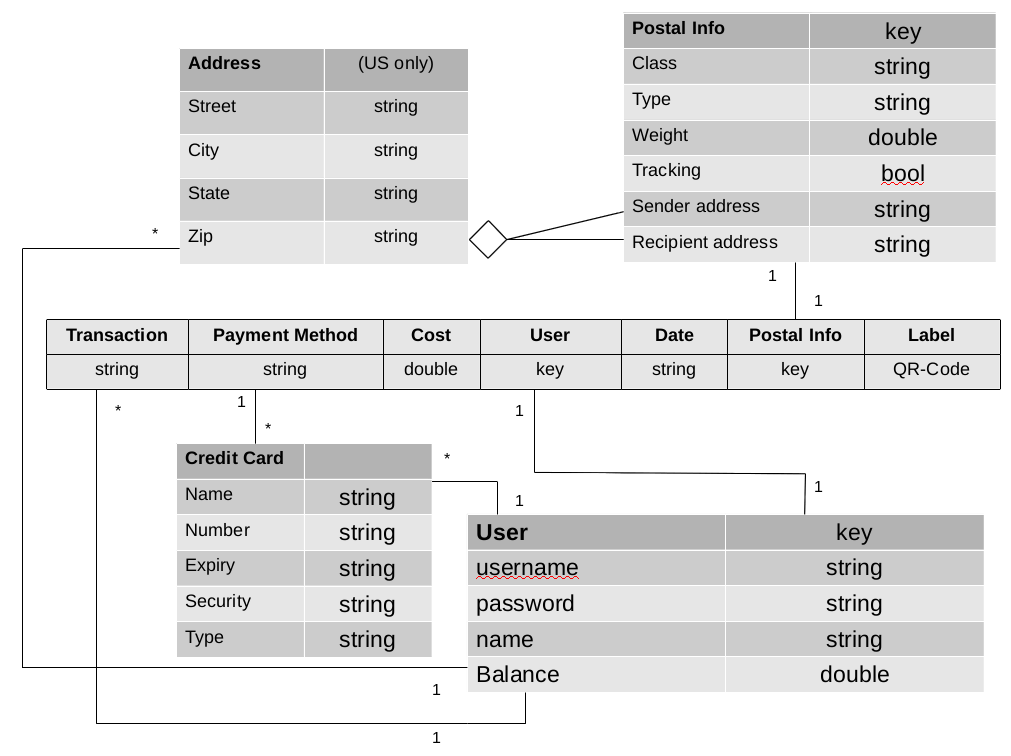
\includegraphics[scale=.4]{3-4-data-structure.png}

\section{Design Constraints}

Constraints for the postage printing website include

\begin{itemize}
\item Able to support PC, Mac platforms.
\item System logs out user after ten minutes of inactivity.
\item System supports all web browsers.
\end{itemize}

\section{Software System Attributes}

The requirements in this section specify the required reliability,
availability, security and maintainability of the software system.

\subsection{Reliability}

For the system to be reliable it will require a stable Internet connection. If
service goes down, it will be restored within 30 minutes. The average failure
rate should be less than 5\% of all transactions.

\subsection{Availability}

The system should not be unavailable for more than 30 minutes within a 24 hour
period, on average.

\subsection{Security}

Users access should be limited to their personal information only. Purchases
should be handled through a secure server to ensure the protection of the
user’s credit card and personal information.

\subsection{Maintainability}

Any updates or fixes shall be able to be made on server-side only, without any
requirements of the user.

\subsection{Portability}

Nothing required.

% add other chapters and sections to suit
\end{document}
